\documentclass[11pt]{article}
\usepackage[T1]{fontenc}
\usepackage[margin=1in]{geometry}
\usepackage{amsmath,amssymb,amsthm}
\usepackage{graphicx}
\usepackage[hidelinks]{hyperref}

\newtheorem{theorem}{Theorem}
\newtheorem{proposition}{Proposition}
\newtheorem{corollary}{Corollary}
\newtheorem{remark}{Remark}

\newcommand{\N}{\mathbb N}
\newcommand{\Tr}{\operatorname{Tr}}
\newcommand{\Span}{\operatorname{span}}
\newcommand{\Sp}{S_p}

\title{Sharp Covering-Index Decay for Schatten Classes}
\author{Automatic Math Discovery Run \texttt{fa\_banach\_001}}
\date{June 16, 2026}

\begin{document}
\sloppy
\maketitle

\section*{Status}

This packet records a \textbf{full result for the Schatten-class
covering-index decay problem} left open in Kania--Ma\'slany, \emph{Raja's
covering index of \(L_p\) spaces}, arXiv:2512.13249.  It also records the
optimal AUS power exponent of \(S_p\).  The result is limited to the classical
Schatten classes \(S_p(H)=L_p(B(H),\Tr)\), not arbitrary non-commutative
\(L_p(M,\tau)\) spaces.

\section*{Source Passage}

The source paper notes in Remark 5.3 that for \(M=B(H)\) the non-commutative
\(L_p(M,\tau)\) space is the Schatten class \(S_p\), records the lower bound
\(\Theta_{S_p}(n)\gtrsim n^{-1/r}\), \(r=\min\{p,2\}\), and then says that
upper bounds are not pursued:

\begin{center}
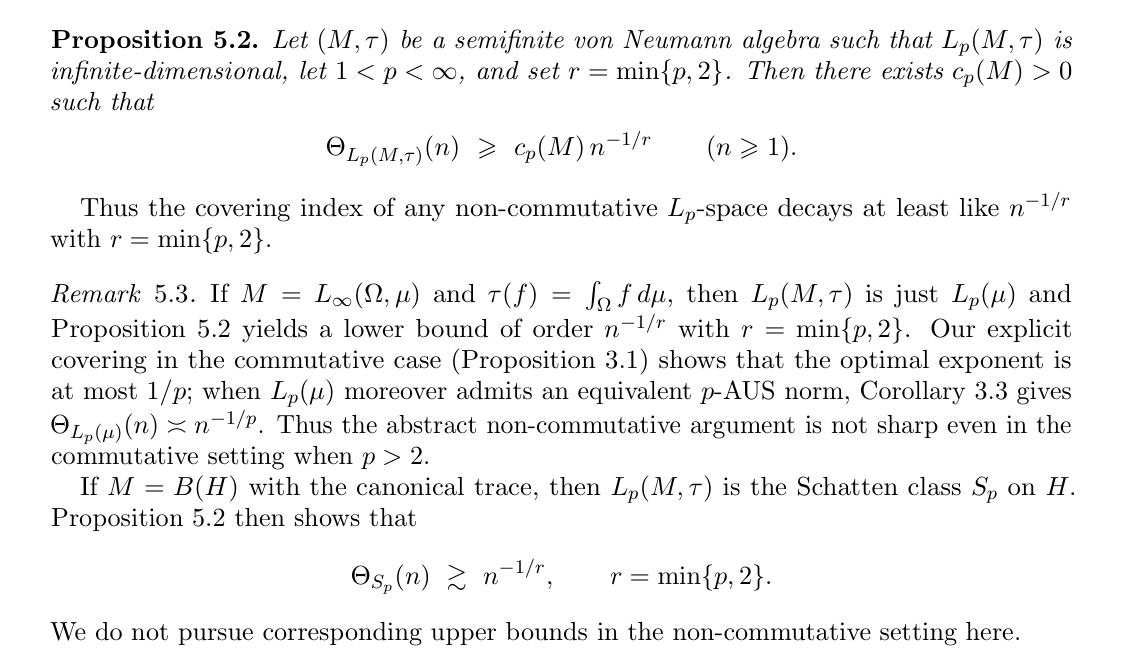
\includegraphics[width=\textwidth]{figures/noncommutative_schatten_gap_crop.png}
\end{center}

The appendix then states the remaining sharp-decay problem explicitly:

\begin{center}

\includegraphics[width=\textwidth]{figures/open_problem_crop.png}
\end{center}

\section*{Definitions}

For a Banach space \(X\), the essential inradius of a set \(A\subseteq X\) is
\[
  \varrho(A)=
  \sup\{r>0:\exists x\in A,\ \exists Y\le X\text{ finite codimensional},
  \ x+r(B_X\cap Y)\subseteq A\}.
\]
Raja's covering index is
\[
  \Theta_X(n)=
  \inf\left\{
  \max_{1\le k\le n}\varrho(A_k):
  B_X=\bigcup_{k=1}^n A_k,\ A_k\text{ closed, convex, bounded}
  \right\}.
\]

Let \(H\) be an infinite-dimensional Hilbert space.  The Schatten class
\(S_p(H)\), \(1\le p<\infty\), is the space of compact operators \(T\) on
\(H\) whose singular-value sequence belongs to \(\ell_p\), with norm
\(\|T\|_p=(\Tr |T|^p)^{1/p}\).

\section*{Proof Intuition}

There are two complementary mechanisms.  The upper bound is a matrix version
of the scalar \(L_p\) block cover from the source paper.  Split
\[
  H=H_1\oplus\cdots\oplus H_n
\]
and cover the unit ball according to which diagonal corner
\(P_kTP_k\) has small \(S_p\)-norm.  Pinching onto diagonal corners is
contractive, so one corner must have norm at most \(n^{-1/p}\).  The
finite-codimensional inradius test is defeated by placing a rank-one operator
far out in that corner, chosen to annihilate the finitely many functionals
defining the subspace.

The lower bound is shorter.  The diagonal operators form a 1-complemented copy
of \(\ell_p\) inside \(S_p(H)\).  The source paper records that covering index
is monotone for contractively complemented subspaces, and it also gives the
sharp scalar estimate \(\Theta_{\ell_p}(n)\asymp n^{-1/p}\) for
\(1<p<\infty\).  Hence \(S_p(H)\) cannot have faster covering-index decay than
the diagonal \(\ell_p\) part.

\section*{Sharp Covering-Index Decay}

\begin{theorem}\label{thm:schatten-upper}
Let \(H\) be an infinite-dimensional Hilbert space and let
\(1\le p<\infty\).  Then for every \(n\in\N\),
\[
  \Theta_{S_p(H)}(n)\le n^{-1/p}.
\]
Indeed, \(B_{S_p(H)}\) has a cover by \(n\) closed convex sets, each of
essential inradius exactly \(n^{-1/p}\).
\end{theorem}

\begin{proof}
Fix \(n\in\N\), and write
\[
  H=H_1\oplus\cdots\oplus H_n
\]
as an orthogonal direct sum of infinite-dimensional closed subspaces.  Let
\(P_k\) be the orthogonal projection onto \(H_k\), and define
\[
  C_k(T)=P_kTP_k,\qquad T\in S_p(H).
\]
Put \(a=n^{-1/p}\), and define
\[
  A_k=\{T\in B_{S_p(H)}:\|C_k(T)\|_p\le a\}\qquad(1\le k\le n).
\]
Each \(A_k\) is closed, convex, and bounded.

Let \(E(T)=\sum_{k=1}^n P_kTP_k\) be the finite pinching.  If
\(U_\varepsilon=\sum_{k=1}^n \varepsilon_k P_k\) for
\(\varepsilon=(\varepsilon_1,\dots,\varepsilon_n)\in\{-1,1\}^n\), then
\[
  E(T)=2^{-n}\sum_{\varepsilon\in\{-1,1\}^n}
  U_\varepsilon T U_\varepsilon .
\]
Since the Schatten norm is unitarily invariant and convex, \(\|E(T)\|_p\le
\|T\|_p\).  Since \(E(T)\) is block diagonal,
\[
  \|E(T)\|_p^p=\sum_{k=1}^n \|C_k(T)\|_p^p.
\]
Thus if \(\|T\|_p\le1\), at least one \(\|C_k(T)\|_p\) is at most
\(n^{-1/p}\), and \(B_{S_p(H)}=\bigcup_k A_k\).

Also \(aB_{S_p(H)}\subseteq A_k\), so \(\varrho(A_k)\ge a\).

We prove the reverse inequality.  Fix \(k\).  Suppose that
\(T\in A_k\), \(Y\le S_p(H)\) is finite codimensional, and \(r>a\).  We shall
find \(W\in B_{S_p(H)}\cap Y\) such that \(T+rW\notin A_k\).  Set
\(V=C_k(T)\), so \(\|V\|_p\le a\).

Choose functionals \(\Phi_1,\dots,\Phi_m\in S_p(H)^*\) with
\[
  Y=\bigcap_{j=1}^m \ker \Phi_j.
\]
By the standard trace-duality representation of Schatten functionals, and
using \(S_1(H)^*=B(H)\) when \(p=1\), there are operators \(B_j\in B(H)\) such
that for rank-one operators
\(\theta_{u,v}(\xi)=\langle \xi,v\rangle u\) one has
\[
  \Phi_j(\theta_{u,v})=\langle B_j u,v\rangle .
\]

Let \(R\le P_k\) be a finite-rank orthogonal projection on \(H_k\).  Since
\(V\in S_p(H_k)\), finite-rank compressions approximate \(V\) in \(S_p\)-norm;
hence \(R\) may be chosen so that
\[
  \bigl(\|RVR\|_p^p+r^p\bigr)^{1/p}
  -\|V-RVR\|_p
  > a. \tag{1}
\]
Indeed, the left side tends to \((\|V\|_p^p+r^p)^{1/p}>r>a\).

The subspace \(K=H_k\ominus R(H_k)\) is infinite-dimensional.  Pick a unit
vector \(u\in K\), then pick a unit vector
\[
  v\in K\cap \Span\{B_1u,\dots,B_mu\}^{\perp}.
\]
This is possible because only finitely many vectors are excluded.  Put
\(W=\theta_{u,v}\).  Then \(W\) is supported in the \(k\)-th corner,
\(\|W\|_p=1\), and \(\Phi_j(W)=0\) for every \(j\), so \(W\in Y\).

Since \(RVR\) acts on \(R(H_k)\) and \(W\) acts from \(K\) to \(K\), the
operator \(RVR+rW\) is block diagonal.  Hence
\[
  \|RVR+rW\|_p^p=\|RVR\|_p^p+r^p.
\]
Using (1),
\[
  \|C_k(T+rW)\|_p
  =\|V+rW\|_p
  \ge \|RVR+rW\|_p-\|V-RVR\|_p
  >a.
\]
Thus \(T+rW\notin A_k\).  Therefore no finite-codimensional ball of radius
larger than \(a\) is contained in \(A_k\), and \(\varrho(A_k)\le a\).  Since
\(\varrho(A_k)\ge a\), the covering has pieces of essential inradius exactly
\(a\), proving the theorem.
\end{proof}

\begin{theorem}\label{thm:schatten-sharp}
Let \(H\) be an infinite-dimensional Hilbert space and let
\(1<p<\infty\).  Then
\[
  \Theta_{S_p(H)}(n)\asymp n^{-1/p}.
\]
\end{theorem}

\begin{proof}
The upper bound is Theorem~\ref{thm:schatten-upper}.  For the lower bound,
choose an orthonormal sequence \((e_j)\) in \(H\), and let \(D\subset S_p(H)\)
be the diagonal subspace
\[
  D=\left\{\sum_j a_j\, e_j\otimes e_j: (a_j)\in\ell_p\right\}.
\]
Then \(D\) is isometric to \(\ell_p\).  The diagonal conditional expectation
\[
  \mathcal E(T)=\sum_j \langle Te_j,e_j\rangle\, e_j\otimes e_j
\]
is contractive on \(S_p(H)\); equivalently, it is the norm-one conditional
expectation onto the diagonal masa, and it follows by finite pinching and
approximation.  Thus \(D\) is a contractively complemented subspace of
\(S_p(H)\).

Kania--Ma\'slany's monotonicity lemma for contractively complemented subspaces
\cite[Lemma 3.3]{KM2512} gives
\[
  \Theta_{\ell_p}(n)=\Theta_D(n)\le \Theta_{S_p(H)}(n).
\]
Their scalar \(L_p\) estimate, applied to the counting measure, gives
\(\Theta_{\ell_p}(n)\asymp n^{-1/p}\) for \(1<p<\infty\)
\cite[Corollary 3.4 and the preceding remark]{KM2512}.  Therefore
\[
  \Theta_{S_p(H)}(n)\gtrsim n^{-1/p}.
\]
Together with the upper bound, this proves the claimed sharp decay.
\end{proof}

\begin{remark}
The upper-bound theorem also holds for \(p=1\).  The lower-bound argument
reduces the \(p=1\) endpoint to the known scalar value of \(\Theta_{\ell_1}\);
the source paper's non-commutative lower-bound discussion, however, is stated
for \(1<p<\infty\), so the main sharp-decay statement above is formulated in
that same range.
\end{remark}

\section*{Optimal AUS Exponent for \(S_p\)}

\begin{proposition}\label{prop:aus-exponent}
Let \(1<p<\infty\).  The largest AUS power exponent obtainable by an
equivalent norm on \(S_p(H)\) is
\[
  \min\{p,2\}.
\]
\end{proposition}

\begin{proof}
The source paper recalls from the non-commutative Clarkson inequalities that
the usual Schatten norm is \(r\)-AUS for \(r=\min\{p,2\}\)
\cite[Appendix]{KM2512}.  Hence the optimal exponent is at least \(r\).

It remains to exclude any \(q>r\).  AUSability passes to subspaces.  If
\(1<p\le2\) and \(S_p(H)\) admitted an equivalent \(q\)-AUS norm for some
\(q>p\), then the diagonal subspace \(D\cong\ell_p\) would be \(q\)-AUSable.
Raja's lower bound, quoted as Theorem 1.6 in the source paper, would imply
\[
  \Theta_{\ell_p}(n)\gtrsim n^{-1/q}.
\]
This contradicts the scalar estimate \(\Theta_{\ell_p}(n)\asymp n^{-1/p}\),
because \(q>p\).

If \(p\ge2\), fix a unit vector \(e_0\in H\).  The row space
\[
  R=\{\theta_{e_0,u}:u\in H\}\subset S_p(H)
\]
is isometric to the Hilbert space \(H\), since each \(\theta_{e_0,u}\) has the
single singular value \(\|u\|\).  If \(S_p(H)\) were \(q\)-AUSable for some
\(q>2\), then \(H\) would be \(q\)-AUSable.  Raja's lower bound would give
\(\Theta_H(n)\gtrsim n^{-1/q}\), contradicting Kania--Ma\'slany's exact
Hilbert computation \(\Theta_H(n)=n^{-1/2}\) \cite[Theorem 2.2]{KM2512}.

Thus no exponent larger than \(\min\{p,2\}\) is possible.
\end{proof}

\section*{What This Solves and What It Does Not}

For classical Schatten classes, the source paper's open Schatten covering
decay question is resolved: the sharp power is \(1/p\), i.e.
\[
  \Theta_{S_p(H)}(n)\asymp n^{-1/p}\qquad(1<p<\infty).
\]
The packet also gives the precise optimal AUS power exponent,
\(\min\{p,2\}\).  In particular, for \(p>2\), the sharp covering-index decay
is governed by the diagonal \(\ell_p\) subspace rather than by the optimal AUS
exponent \(2\).

The packet does not settle arbitrary non-commutative \(L_p(M,\tau)\) spaces.
The upper-bound proof uses the concrete decomposition of \(H\) into matrix
corners, and the lower-bound proof uses the diagonal \(\ell_p\) masa in
\(B(H)\).

\section*{Verification and Novelty Check}

The proof is abstract and uses no numerical computation.  The code
\texttt{code/make\_open\_problem\_crops.py} renders the two source-passage
crops from \texttt{source\_paper.pdf}.

Local registry, solution, attempt, and proof-gap indexes had only the earlier
partial packet from this run for arXiv:2512.13249, which has now been promoted
and rewritten here.  A bounded web/arXiv search on June 16, 2026 for
``Raja's covering index Schatten \(n^{-1/p}\)'', ``Theta S\_p covering
index'', ``Schatten Raja covering index ell\_p'', and ``essential inradius
S\_p Theta'' found Raja's original paper arXiv:2503.03721 and the source
paper arXiv:2512.13249, but no later paper giving the diagonal lower-bound
upgrade or the resulting sharp Schatten decay.  The source paper itself says
that non-commutative upper bounds are not pursued and that the sharp
Schatten-class decay remains open.

\section*{Revision History}

The first pass on this target produced only the upper bound
\(\Theta_{S_p(H)}(n)\le n^{-1/p}\).  That superseded partial packet is kept
inside this packet at \texttt{history/partial\_upper\_bound/}.  The present
version adds the diagonal \(\ell_p\) lower bound and the optimal AUS exponent
argument, so the indexed durable result is this full packet.

\section*{Human Review Recommendation}

Review as a likely valid full solution of the Schatten covering-index decay
subproblem.  The main checks are the finite-codimensional rank-one tail
argument in Theorem~\ref{thm:schatten-upper}, the use of the diagonal
conditional expectation and complemented-subspace monotonicity in
Theorem~\ref{thm:schatten-sharp}, and the subspace obstruction in
Proposition~\ref{prop:aus-exponent}.

\begin{thebibliography}{9}

\bibitem{KM2512}
T. Kania and N. Ma\'slany,
\emph{Raja's covering index of \(L_p\) spaces}, arXiv:2512.13249.

\bibitem{Raja2503}
M. Raja,
\emph{A covering index for Banach spaces}, arXiv:2503.03721.

\end{thebibliography}

\end{document}
